\section{Response asymmetry and dissipation are distinct observables}
\label{sec:decoupling}

Both $\R$ and $\EPR$ vanish exactly on potential games and read loudly on
harmonic ones, so a natural conjecture (C1 in the programme's ledger) held
that the four meters co-move tightly along the whole family. Marginally they
do: over 1{,}000 games ($100 \times 10$ $\alpha$ levels, $\lambda = 1.2$),
Spearman $\rho(\EPR, \R) = 0.993$.

\begin{finding}[Conditional decoupling and sign reversal; F-0004]
The marginal agreement is $\alpha$-confounding. Conditional on the level,
$\rho(\EPR, \R)$ is $+0.80..+0.88$ for $\alpha \le 0.65$, degrades through
$+0.61$ ($\alpha=0.75$) and $+0.32$ ($\alpha=0.85$), and \emph{reverses} to
$-0.355$ at $\alpha = 0.95$: among near-pure-harmonic games, larger response
asymmetry associates with \emph{less} dissipation
(Figure~\ref{fig:decoupling}). This finding originated as a red-team
objection to our own headline correlation; the stratified metric is now a
permanent artifact field.
\end{finding}

\begin{figure}[t]
\centering
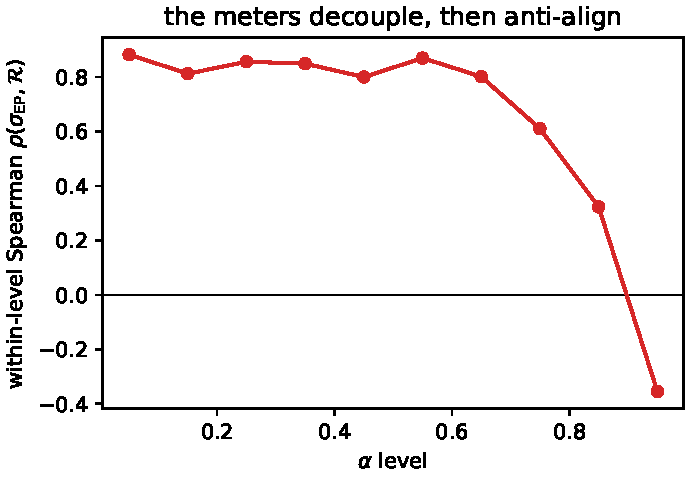
\includegraphics[width=0.55\linewidth]{figures/decoupling.pdf}
\caption{Within-level rank correlation between $\EPR$ and $\R$ along
$\alpha$. Strong coupling while a potential component modulates both meters;
decoupling and sign reversal as it vanishes. Artifact:
\texttt{chain\_comovement.json}.}
\label{fig:decoupling}
\end{figure}

\paragraph{Mechanism, by preregistered test (F-0007).} We proposed a repair:
perhaps only $\R$'s \emph{denominator} $\lVert\chieq + \chieq{}^\top\rVert$
misbehaves at high $\alpha$ (H2), while the antisymmetric numerator keeps
tracking dissipation (H1) --- in which case a numerator-only meter would
restore coupling. On the identical seeded families, paired by game:
\textbf{H2 confirmed} --- at $\alpha=0.95$,
$\rho(\R,\, 1/\lVert\chieq{+}\chieq{}^\top\rVert) = 0.993$, rising
monotonically from $\approx 0$ at low $\alpha$; $\R$'s within-level variation
in the near-harmonic regime is entirely the shrinking symmetric response.
\textbf{H1 refuted} --- the numerator \emph{also} decouples:
$\rho(\lVert\chieq{-}\chieq{}^\top\rVert, \EPR) = -0.37$ at $\alpha = 0.95$,
down from $+0.77..0.86$ at $\alpha \le 0.65$. No renormalisation of the
response matrix recovers the dissipation ordering.

\paragraph{The structural reading.} This negative result is the better
result. $\chieq$ is a \emph{local derivative} of the equilibrium map at the
QRE point; $\EPR$ is a \emph{global functional of the stationary flux} of the
joint-profile chain. They co-vary exactly as long as a potential component
modulates both, and part company when it vanishes. Consequently the
instrument-scope table of \citep{p1} is not a convenience but a necessity:
$\R$ answers ``is this system potential?'' (exactly, at every $\lambda$);
$\EPR$ answers ``how hard is it driven?''; and in the near-harmonic regime
neither substitutes for the other. Conjecture C1 is thereby resolved as:
co-movement for $\alpha \lesssim 0.65$, structural failure above. The
crossover's $\lambda$- and size-dependence (open in v0.1) is now measured
(F-0010): the \emph{collapse} of within-level coupling at $\alpha = 0.95$
is universal --- from $\approx 0.90$ at $\alpha \le 0.65$ to $\le 0.25$
in every condition tested ($\lambda \in \{0.8, 1.2, 2.0\}$, both $3\times
3$ and $4\times 4$) --- while the \emph{negative sign} is a second,
$\lambda$-dependent effect ($+0.25 \to +0.03 \to -0.23$ across the three
$\lambda$; $-0.26$ at $4\times 4$), with each individual sign within
$\sim$2 null-SD at $n = 60$. We record the methodological event plainly:
the initial criterion (reversal in $\ge 3/4$ conditions) \emph{failed} and
the failure is the finding --- the robust fact is decorrelation, not
anti-alignment, and whether the sign tracks depth into the supercritical
wedge is the sharp remaining question.
